% !TeX spellcheck = pl_PL
\documentclass[a4paper,twoside]{article}
\usepackage{polski}
\usepackage[utf8]{inputenc}
\usepackage{graphicx}
\usepackage{amsmath}

\usepackage[unicode, bookmarks=true]{hyperref} %do zakładek
\usepackage{tabto} % do tabulacji
\NumTabs{6} % globalne ustawienie wielkosci tabulacji
\usepackage{array}
\usepackage{multirow}
\usepackage{array}
\usepackage{dcolumn}
\usepackage{bigstrut}


\setlength{\textheight}{24cm}
\setlength{\textwidth}{15.92cm}
\setlength{\footskip}{10mm}
\setlength{\oddsidemargin}{0mm}
\setlength{\evensidemargin}{0mm}
\setlength{\topmargin}{0mm}
\setlength{\headsep}{5mm}

\newcolumntype{M}[1]{>{\centering\arraybackslash}m{#1}}
\newcolumntype{N}{@{}m{0pt}@{}}

\graphicspath{ {./images/} }

\begin{document}
\bibliographystyle{plain}



\begin{titlepage}
\title{\huge Architektura komputerów - ULTIMATE}
\author{\large SonMati \\ Doxus}
\maketitle
\end{titlepage}

%===============================================================================
% *** PYTANIA I ODPOWIEDZI *****************************************************
%===============================================================================
\part*{Pytania i odpowiedzi}
\section{Moc obliczeniowa komputerów wektorowych: {\small /Forczu}}
	\begin{itemize}
    \item Zależy od liczby stopni potoku.\\
    {\small \emph{Moc obliczeniowa nie jest zależna od liczby stopni potoku. Ta jedynie wpływa na ilosć rozkazów jakie mogą być wykonane w chwili czasu w jednostce potokowej.}}
    \item \textbf{Jest odwrotnie proporcjonalna do długości taktu zegarowego}\\
    {\small \emph{Tak, obliczamy ją wzorem} $Przep=lim_{n \to \infty}\frac{n}{t_{start}+(n-1)\times\tau}=\frac{1}{\tau}$}
    \item Jest wprost proporcjonalna do długości taktu zegarowego\\
    {\small \emph{Nie, patrz wyżej.}}
    \item Zależy odwrotnie proporcjonalnie od liczby jednostek potokowych połączonych łańcuchowo.\\
    {\small \emph{Nie, idea operacji wektorowej na komputerze wektorowym zakłada jedną jednostkę potokową. Ich zwiększenie nie powinno wpłynąć bezposrednio na moc.}}
    \item \textbf{Zmierza asymptotycznie do wartości maksymalnej wraz ze wzrostem długości wektora}\\
    {\small \emph{Tak, istnieje pewna wartosć maksymalna do której moc dąży logarytmicznie wraz ze wzrostem długosci wektora.}}
    \item Nie zależy od długości wektora\\
    {\small \emph{Bzdura, patrz wyżej.}}
    \item Zależy liniowo od długości wektora\\
    {\small \emph{Bzdura, patrz wyżej.}}
    \end{itemize}

\section{Czy poniższa lista jest rosnąco uporządkowana według skalowalności:}
	\begin{itemize}
    \item Systemy ściśle połączone, systemy ze wspólną pamięcią, systemy SMP
    \item \textbf{Systemy ze wspólna magistralą, systemy wielomagistralowe, systemy z przełącznicą krzyżową}
    \item Systemy SMP, systemy z pamięcią wieloportową, systemy z przełącznicą krzyżową
    \item NUMA, MPP, SMP
    \item \textbf{Systemy z pamięcią wspólną, systemy o niejednorodnym dostępie do pamięci, z pamięcią rozproszoną}
    \item Systemy SMP, NUMA, klastry, UMA
    \item \textbf{Systemy symetryczne, o niejednorodnym dostępie do pamięci, systemy z przesyłem komunikatów}
    \end{itemize}
    
\section{Komputery macierzowe {\small /Forczu}}
	\begin{itemize}
    \item \textbf{Mają w liście rozkazów m.in. rozkazy operujące na wektorach danych}\\
    {\small \emph{Tak, te komputery są rozwinięciem komputerów wektorowych i muszą mieć rozkazy wektorowe. Komputery macierzowe posiadają po \emph{n} jednostek przetwarzających, które potrafią razem obliczyć \emph{n} składowych wektora.}}
    \item Mają macierzowe potokowe układy arytmetyczne\\
    {\small \emph{Nie, posiadają natomiast jednostki przetwarzające. Z kolei potokową jednostkę arytmetyczną posiadają komputery wektorowe.}}
    \item Mają w typowych rozwiązaniach zestaw pełnych procesów połączonych siecią połączeń\\
    {\small \emph{Nie, w typowym rozwiązaniu jest jeden pełny procesor z wieloma jednostkami potokowymi, które są połączone siecią łączącą (statyczną lyb dynamiczną). Sieć połączeń pełnych procków posiadają superkomputery z top500 (Nie jestem pewien tej odpowiedzi).}}
    \item \textbf{Wykonują synchroniczną operację wektorową w sieci elementów przetwarzających}\\
    {\small \emph{Tak własnie działają.}}
    \end{itemize}
    
\section{Przetwarzanie potokowe {\small /Forczu}}
	\begin{itemize}
    \item Nie jest realizowane dla operacji zmiennoprzecinkowych\\
    {\small \emph{Nie ma takiego ograniczenia. Przetwarzanie potokowe dotyczy optymalizacji czasu wykonywania rozkazów - podziału realizacji rozkazu na fazy. Owszem, dla argumentów zmiennoprzecinkowym mogą wystąpić problemy związane z czasem obliczeń (uniemożliwienie wykonania rozkazu w jednym takcie), co oże zablokować napełnianie potoku, jednak nie uniemożliwia to zastosowania potoku. /Forczu}}
    \item Nie jest realizowane w procesorach CISC\\
    {\small \emph{Przetwarzanie potokowe znalazło zastosowanie głównie w architekturze RISC, jednak CISC też z niej korzysta. Przykłady: VAX 11/780 (CISC), Ultra SPARC III (RISC)}.}
    \item \textbf{Daje przyspieszenie nie większe od liczby segmentów (stopni) jednostki potokowej}\\
    {\small \emph{Tak, przyspieszenie jest stosunkiem czasu wykonywania \emph{n} rozkazów dla procesora niepotokowego oraz czasu dla procesora potokowego. W idealnym przypadku, gdy każdy stopień dzieli okres rozkazu po równo, a liczba rozkazów dąży do nieskończoności, stosunek ten jest równy P - ilości stopni.}}
    \item W przypadku wystąpienia zależności między danymi wywołuje błąd i przerwanie wewnętrzne.\\
    {\small \emph{Hm, dobre pytanie. Tak, zależnosci danych mogą wystapić (zjawisko hazardu) i rozdupić program, ale po to własnie istnieją mechanizmy by temu zapobiegać. Każda szanująca się architektura to potrafi: albo sprzętowo, albo na etapie kompilacji, która modyfikuje i optymalizuje program. A jeżeli po modyfikacji pewien rozkaz nie wykona się w jednym takcie, napełnianie potoku jest przerywane (ale błędu chyba nie wywala), patrz wyżej.}}
    \item Jest realizowane tylko dla operacji zmiennoprzecinkowych\\
    {\small \emph{Pfff, no chyba nie XD Jest realizowane dla każdego rodzaju rozkazu.}}
    \end{itemize}

% --- PYTANIE 5
\section{W procesorach superskalarnych {\small /Forczu}}
	\begin{itemize}
    \item \textbf{Liczba rozkazów, które procesor może wykonać w 1 takcie zależy od liczby jednostek potokowych w procesorze}\\
    {\small \emph{Procesory superskalarne posiadają wiele jednostek potokowych, które są konieczne by móc wykonywać wiele rozkazów w jednym takcie. Od ich liczby zależy owa liczba rozkazów.}}
    \item Liczba rozkazów, które procesor może wykonać w jednym takcie, zależy od liczby stopni potoku.\\
    {\small \emph{Nie, liczba stopni potoku mówi, na ile częsci dzieli się dany rozkaz w tej jednostce potokowej. One umożliwiają wykonanie wielu rozkazów w jednej jednostce czasu, jednak nie przekłada się to bezposrednio na liczbę rozkazów, ze względu na zawikłania czasowe, oraz nie jest to idea procesora superskalarnego.}}
    \item Liczba rozkazów pobieranych z pamięci, w każdym takcie musi przekraczać liczbę jednostek potokowych\\
    {\small \emph{Liczba pobranych rozkazów powinna być co najmniej równa ilosci jednostek potokowych.}}
    \item \textbf{Liczba rozkazów, które procesor może wykonać w taktach zależy od liczby jednostek potokowych w procesorze}\\
    {\small \emph{Tak, patrz pierwsza odpowiedź.}}
    \end{itemize}

\section{Systemy SMP}
	\begin{itemize}
    \item Wykorzystują protokół MESI do sterowania dostępem do wspólnej magistrali
    \item Posiadają skalowalne procesory
    \item Posiadają pamięć fizycznie rozproszoną, ale logicznie wspólną
    \end{itemize}

\section{Komputery wektorowe}
	\begin{itemize}
    \item Posiadają jednostki potokowe o budowie wektorowej\\
    {\small \emph{Nie, posiadają potokowe jednostki arytmetyczne, które nie są wektorowe.}}
    \item \textbf{Posiadają w liście rozkazów m.in. rozkazy operujące na wektorach danych}\\
    {\small \emph{Jak najbardziej, nie mogłyby się bez tego obejsć.}}
    \item \textbf{Wykorzystują od kilku do kilkunastu potokowych jednostek arytmetycznych}\\
    {\small \emph{Tak, tych jednostek może być wiele, można to zauważyć na przykładzie komputera Cray-1 (wykład 7-8, slajd 31)}}
    \item Posiadają listę rozkazów operujących wyłącznie na wektorach\\
    {\small \emph{Zdecydowanie nie. Owszem, te komputery posiadają rejestry wektorowe i wektorowe jednostki zmiennoprzecinkowe, ale nie jest to wszystko. Mają również normalne rejestry, adresację, jednostki skalarne i możliwosć wykonywania na nich operacji.}}
    \end{itemize}

\section{Procesory wektorowe}
	\begin{itemize}
    \item \textbf{Mogą być stosowane w systemach wieloprocesorowych}
    \item \textbf{Mają listę rozkazów operującą jedynie na wektorach}
    \item \textbf{Mają moc kilka razy większą od procesorów skalarnych}
    \end{itemize}

\section{Systemy MPP są zbudowane z węzłów którymi mogą być}
	\begin{itemize}
    \item \textbf{Systemy SMP}
    \item Klastry
    \item Konstelacje
    \item \textbf{Systemy NUMA}
    \item \textbf{Procesory}
    \end{itemize}

% --- PYTANIE 10
\section{W architekturze NUMA}
	\begin{itemize}
    \item \textbf{Dane są wymieniane między węzłami w postaci linii pamięci podręcznej (PaP)}
    \item Spójność PaP węzłów jest utrzymywana za pomocą protokołu MESI
    \item Czas dostępu do pamięci lokalnej w węźle jest podobny do czasu dostępu do pamięci nielokalnej
    \item \textbf{Czas zapisu danych do pamięci nielokalnej może być znacznie dłuższy od czasu odczytu z tej pamięci}
    \item \textbf{Każdy procesor ma dostęp do pamięci operacyjnej każdego węzła}
    \item Procesy komunikują się poprzez przesył komunikatów
    \item \textbf{Pamięć operacyjna jest rozproszona fizycznie pomiędzy węzłami, ale wspólna logicznie}
    \end{itemize}

\section{Mechanizmy potokowe stosowane są w celu {\small /Forczu}}
	\begin{itemize}
    \item Uszeregowania ciągu wykonywanych rozkazów\\
    {\small \emph{Nie, zupełnie nie o to chodzi. Ciąg może zostać uszeregowany przez kompilator w celu optymalizacji. Jednak celem tego mechanizmu jest zrównoleglenie wykonywania rozkazów -> zmiana kolejnosci ich realizacji nie jest założeniem.}}
    \item \textbf{Uzyskania równoległej realizacji rozkazów}
    {\small \emph{No tyć. Potoki umożliwiają realizację wielu rozkazów jednoczesnie dzieląc jednostkę centralną na wg stopni, jak np. pobranie rozkazu i wykonania rozkazu. Dzięki temu dwa rozkazy mogą wykonywać się jednoczesnie, oba w innych fazach.}}
    \item \textbf{Przyspieszenia realizacji rozkazów}\\
    {\small \emph{Tak, to główny cel. Umożliwienie wykonania rozkazów umożliwia przyspieszenie, które oblicza się jako stosunek czasu wykonywania rozkazów w procesorze niepotokowym do czasu realizacji w procesorze potokowym. W idealnym przypadku jest ono równe \emph{P} - ilości podziałów / stopni / faz / zwał jak zwał.}}
    \end{itemize}

\section{Protokół MESI}
	\begin{itemize}
    \item Jest wykorzystywany do sterowania dostępem do magistrali w systemie SMP
    \item \textbf{Zapewnia spójność pamięci cache w systemie SMP}
    \item Służy do wymiany komunikatów w systemie MPP
    \item Chroni przed hazardem w proc superskalarnych
    \end{itemize}
    
\section{Mechanizm skoków opóźnionych {\small /Forczu}}
	\begin{itemize}
    \item \textbf{Polega na opóźnianiu wykonywania skoku do czasu wykonania rozkazu następnego za skokiem}\\
    {\small \emph{Tak, cały ten mechanizm sprowadza się do opóźnienia efektu skoku o jeden rozkaz. Zapewnia to, że rozkaz następny po skoku zawsze będzie wykonywany w całosci.}}
    \item Wymaga wstrzymania potoku na jeden takt.\\
    {\small \emph{Nie, mechanizm potoków nie musi być wstrzymywany. Mechanizm ten zmienia postać programu w trakcie kompilacji, ale na samą realizację potoku nie ma wpływu (afaik, not sure).}}
    \item Powoduje błąd na końcu pętli\\
    {\small \emph{Pfff, jak programista ssie pałę to tak, jednak w założeniu tak się nie dzieje.}}
    \item \textbf{Wymaga umieszczenia rozkazu NOP za rozkazem skoku lub reorganizacje programu}.\\
    {\small \emph{Tak, mechanizm sprowadza się do tego, i tylko do tego, patrz pierwsza odpowiedź.}}
    \end{itemize}
    
\section{Charakterystyczne cechy architektury MPP}
	\begin{itemize}
    \item Spójność pamięci podręcznej wszystkich węzłów
    \item \textbf{Fizycznie rozproszona PaO}
    \item Fizycznie rozproszona PaO, ale logicznie wspólna
    \item \textbf{Przesył komunikatów między procesorami}
    \item Niska skalowalność
    \item Jednorodny dostęp do pamięci wszystkich węzłów
    \end{itemize}

% --- PTYTANIE 15
\section{Jak można ominąć hazard danych {\small /Forczu}}
	\begin{itemize}
    \item Poprzez rozgałęzienia\\
    {\small \emph{Nie, to jest stosowane do usuwania hazardu sterowania związanego ze skokami i rozgałęzieniami.}}
    \item Poprzez uproszczenie adresowania - adresowanie bezpośrednie.\\
    {\small \emph{Bullshit. Nie wiem w czym miało by pomóc uproszczenia adresowania, poza pójsciem w stronę RISCu, ale na hazard to nie pomoże.}}
    \item \textbf{Przez zamianę rozkazów}\\
    {\small \emph{Tak, i na tym polega mechanizm skoków opóźnionych, które mogą program zmodyfikować (dodać rozkaz NOP) albo zoptymalizować, własnie zamieniają rozkazy kolejnoscią.}}
    \end{itemize}

\section{Cechy architektury CISC {\small /Forczu}}
	\begin{itemize}
    \item Czy może być wykonana w VLIW\\
    {\small \emph{Nie, architektura VLIW dotyczy mikroprocesorów i miała na celu jak największe zmniejszenie jednostki centralnej i jej rozkazów (RISC)}. }
    \item \textbf{Czy występuje model wymiany danych typu pamięć - pamięć}\\
    {\small \emph{Tak, posiada róznież niewielką ilosc rejestrow.}}
    \item Jest mała liczba rozkazów\\
    {\small \emph{Nie, w tej architekturze jest PEŁNA (complex) lista rozkazów. Niektóre z zaawansowanych pleceń nawet nie były wykorzystywane, i bum! tak powstał RISC.}}
    \end{itemize}

\section{Cechy architektury RISC {\small /Forczu}}
	\begin{itemize}
    \item \textbf{Czy występuje model wymiany danych typu rej-rej}\\
    {\small \emph{Tak, a komunikacja z pamięcią operacyjną odbywa się wyłącznie za pomocą rozkazów LOAD i STORE}}
    \item \textbf{Jest mała liczba trybów adresowania}\\
    {\small \emph{Tak, raptem 4 w procesorze RISC I podczas gdy CISCi mogą mieć ich kilkanascie, w tym takie bardzo złożone.}}
    \item \textbf{Jest wykonywanych kilka rozkazów w jednym takcie}\\
    {\small \emph{Tu jest haczyk - pierwszy procesor RISC I (1980) stawiał sobie za cel wykonanie \emph{jednego rozkazu w jednym takcie} i dokładnie tak brzmiało jego założenie projektowe. Jednak jego fizyczna realizacja (1982) posiadała dwustopniowy potok.}}
    \item \textbf{Jest wykonywanych kilka rozkazów w jednym takcie (w danej chwili czasu)}\\
    {\small \emph{Chodzi o przetwarzanie potokowe. Patrz wyżej + w wykładach jako cecha tej architektury jest napisane "Intensywne wykorzystanie przetwarzania potokowego", co odnosi się do faktu, że obecnie nie ma procesora typu RISC, który go nie ma. Wg mnie prawda.}}
    \item Jest wykonywanych kilka instrukcji procesora w jednym rozkazie asemblerowym\\
    {\small \emph{Nic mi na ten temat nie wiadomo. Brzmi jednak zbyt hardo i odlegle od tematu zmniejszania ilosci rozkazów.}}
    \item \textbf{Układ sterowania w postaci logiki szytej}\\
    {\small \emph{Tak.}}
    \end{itemize}

\section{Przepustowość (moc obliczeniowa) dużych komputerów jest podawana w}
	\begin{itemize}
    \item \textbf{GFLOPS}
    \item Liczbie instrukcji wykonywanych na sekundę
    \item \textbf{Liczbie operacji zmiennoprzecinkowych na sekundę}
    \item Mb/sek
    \end{itemize}

\section{Podstawą klasyfikacji Flynna jest {\small /Forczu}}
	\begin{itemize}
    \item Liczba jednostek przetwarzających i sterujących w systemach komputerowych
    \item Protokół dostępu do pamięci operacyjnej
    \item \textbf{Liczba strumieni rozkazów i danych w systemach komputerowych}
    \item Liczba modułów pamięci operacyjnej w systemach komputerowych\\\\
    {\small \emph{To po prostu należy zapamiętać. \textbf{Kryterium klasyfikacji Flynna jest \emph{liczba strumieni rozkazów} oraz \emph{liczba strumieni danych} w systemie komputerowym. NIC WIĘCEJ, NIC MNIEJ.\\
    Albo inaczej: \emph{$Liczba\_strumieni\times(rozkazow+danych)$}}}}
    \end{itemize}

% --- PYTANIE 20
\section{Rozkazy wektorowe mogą być realizowane przy wykorzystaniu  {\small /Forczu}}
	\begin{itemize}
    \item \textbf{Macierzy elementów przetwarzających}\\
    {\small \emph{Tak, komputery macierzowe operują na rozkazach wektorowych.}}
    \item Zestawu procesorów superskalarnych\\
    {\small \emph{Procesory superskalarne w założeniu nie posiadają rozkazów wektorowych.}}
    \item \textbf{Technologii MMX}\\
    {\small \emph{Tak, jest to pochodna technologia modelu SIMD, wykonuje operacje na krótkich wektorach (64-bit)}}
    \item Sieci połączeń typu krata\\
    {\small \emph{Jest to sieć połączeń, która łączy jednostki przetwarzające w komputerze macierzowym. Raczej na wektorach na częsć komputera nie działa.}}
    \item \textbf{Potokowych jednostek arytmetycznych}\\
    {\small \emph{Tak, takie znajdują się w komputerach wektorowych.}}
    \end{itemize}

\section{Architektura superskalarna {\small /Forczu}}
	\begin{itemize}
    \item Dotyczy systemów SMP\\
    {\small \emph{Zdecydowanie nie tylko. Architektura superskalarna wymaga mechanizmu potokowego, czyli dotyczy głównie architektury RISC.}}
    \item Wymaga zastosowania protokołu MESI\\
    {\small \emph{Nie, architektura superskalarna wymaga jedynie zastosowania co najmniej dwóch jednostek potokowych.}}
    \item \textbf{Umożliwia równoległe wykonywanie kilku rozkazów w jednym procesorze}\\
    {\small \emph{Tak, i taki jest cel jej istnienia. Umożliwia to mechanizm potokowy.}}
    \item Wywodzi się z architektury VLIW\\
    {\small \emph{Wręcz odwrotnie, to VLIW wykorzystuje architekturę superskalarną na której opiera swój podział rozkazów na paczki.}}
    \end{itemize}

\section{Klastry}
	\begin{itemize}
    \item Mają średnią skalowalność
    \item Wykorzystują model wspólnej pamięci
    \item \textbf{W węzłach mogą wykorzystywać systemy SMP}
    \item \textbf{Do komunikacji między procesami wykorzystują przesył komunikatów}
    \item Wykorzystują przełącznicę krzyżową jako sieć łączącą węzły
    \item \textbf{W każdym węźle posiadają pełną instalację systemu operacyjnego}
    \end{itemize}

\section{Pojęcie równoległości na poziomie rozkazów: {\small /Forczu}}
	\begin{itemize}
    \item Dotyczy architektury MIMD\\
    {\small \emph{Nie, dotyczy ona mechanizmów potokowych (CISC i RISC), architektury superskalarnej oraz VLIW.}}
    \item \textbf{Odnosi się m.in. do przetwarzania potokowego}\\
    {\small \emph{Tak, ideą mechanizmu potoków jest zrównoleglenie rozkazów i możliwosć wykonywania wielu z nich w tej samej chwili czasu.}}
    \item Dotyczy architektury MPP\\
    {\small \emph{Nie, patrz wyżej.}}
    \item \textbf{Dotyczy m.in. architektury superskalarnej}\\
    {\small \emph{Tak, patrz wyżej.}}
    \end{itemize}

\section{Systemy wieloprocesorowe z pamięcią wspólną}
	\begin{itemize}
    \item Zapewniają jednorodny dostęp do pamięci
    \item \textbf{Mogą wykorzystywać procesory CISC}
    \item \textbf{Są wykorzystywane w klastrach}
    \item Wykorzystują przesył komunikatów między procesorami
    \item \textbf{Wykorzystują katalog do utrzymania spójności pamięci podręcznych}
    \end{itemize}

% --- PYTANIE 25
\section{Hazard danych {\small /Forczu}}
	\begin{itemize}
    \item \textbf{Czasami może być usunięty przez zmianę kolejności wykonania rozkazów}\\
    {\small \emph{Tak, służy do tego mechanizm skoków opóżnionych, który odbywa się na poziomie kompilacji programu.}}
    \item Nie występuje w architekturze superskalarnej
    \item Jest eliminowany przez zastosowanie specjalnego bitu w kodzie programu\\
    {\small \emph{Nic mi o tym nie wiadomo. Pewne dodatkowe bity są wykorzystywane w mechaniźmie przewidywania rozgałęzień, który służy do eliminacji hazardu, jednak on to odbywa się PRZED realizacją programu i sprowadza się do zmiany kolejnosci wykonywania rozkazów przez kompilator. Nic nie dodaje do tresci programu.}}
    \item Może wymagać wyczyszczenia potoku i rozpoczęcia nowej (…)\\
    {\small \emph{Nie wiem jak hazard danych może czegokolwiek wymagać skoro jest zjawiskiem ubocznym i je eliminujemy. Jeżeli jednak chodzi o metody eliminacji hazardu, jak mechanizmy skoków opóźnionych lub przewidywania rozgałęzień, nie wymagają czyszczenia potoku. Sprzetowa i programowa eliminacja hazardu jedynie może doprowadzić do \textbf{wstrzymania} napełniania potoku.}}
    \end{itemize}

\section{Przetwarzanie wielowątkowe {\small /Forczu}}
	\begin{itemize}
    \item \textbf{Zapewnia lepsze wykorzystanie potoków}\\
    {\small \emph{Tak, ma na celu minimalizację strat cykli w trakcie realizacji wątku, jakie mogą powstać na wskutek:
    		\begin{itemize}
    			\item chybionych odwołań do pamięci podręcznej
    			\item błędów w przewidywaniu rozgałęzień
    			\item zależności między argumentami
    		\end{itemize}}}
    \item \textbf{Minimalizuje straty wynikające z chybionych odwołań do pamięci podręcznej}\\
    {\small \emph{Tak, patrz wyżej.}}
    \item \textbf{Wymaga zwielokrotnienia zasobów procesora (rejestry, liczniki rozkazów, itp.)}\\
    {\small \emph{Niestety tak, jest to warunek sprzętowej realizajci wielowątkowosci.}}
    \item Nie może być stosowane w przypadku hazardu danych\\
    {\small \emph{Nie, hazard danych wynika z zależnosci między argumentami, które są naturalnym ryzykiem przy stosowaniu mechanizmu potokowego. Nie powinny być blokowane z tego powodu, tym bardziej, że wielowątkowosć ma dodatkowo chronić liczbę cykli przed zgubnym wpływem hazardu.}}
    \end{itemize}

\section{Okna rejestrów {\small /Forczu}}
	\begin{itemize}
    \item Chronią przez hazardem danych\\
    {\small \emph{Lolnope, od tego są mechanizmy skoków opóźnionych i przewidywania rozgałęzień. Okno rejestrów zapewnia ciągłe i optymalne wykonywanie procedur.}}
    \item \textbf{Minimalizują liczbę odwołań do pamięci operacyjnej przy operacjach wywołania procedur}\\
    {\small \emph{Tak, dokładnie do tego one służą. Rejestr niski procedury A staje się rejestrem wysokim procedury B itd. Innymi słowy, procedura A wywołuje procedurę B, i tak dalej. I po cos w tym wszystkim są rejestry globalne.}}
    \item Są charakterystyczne dla architektury CISC\\
    {\small \emph{Nie, zostały zaprojektowane specjalnie dla architektury RISC. Jako pierwszy posiadał je procesor RISC I.}}
    \item Są zamykane po błędnym przewidywaniu wykonania skoków warunkowych.\\
    {\small \emph{W mechanizmie prognozowania rozgałęzień jest możliwosć błędnego przewidywania. Jednak błędna prognoza powoduje tylko zmianę strategii (przewidywanie wykonania lub niewykonania), a nie zamykanie okna.}}
    \item \textbf{Są przesuwane przy operacjach wywołania procedur}\\
    {\small \emph{Tak, z każdą nową wywołaną procedurą okno rejestrów przesuwane jest w dół (ze 137 do 0)}}
    \end{itemize}

\section{Tablica historii rozgałęzień {\small /Forczu}}
	\begin{itemize}
    \item \textbf{Zawiera m.in. adresy rozkazów rozgałęzień}\\
    {\small \emph{Tak, tablica ta zawiera bit ważnosci, \emph{adres rozkazu rozgałęzienia}, bity historii oraz \emph{adres docelowy rozgałęzienia}.}}
    \item \textbf{Pozwala zminimalizować liczbę błędnych przewidywań rozgałęzień w zagnieżdżonej pętli}\\
    {\small \emph{Tak, z tego co wiem jest strategią dynamiczną i najbardziej optymalną ze wszystkich - skończony automat przewidywania rozgałęzień oparty na tej tablicy (z dwoma bitami historii) może być zarealizowany na dwóch bitach.}}
    \item Nie może być stosowana w procesorach CISC\\
    {\small \emph{Ten mechanizm służy zabezpieczeniu przed hazardem, który występuje w przetwarzeniu potokowym, a z tego korzystają zarówn CISC jak i RISC.}}
    \item Jest obsługiwana przez jądro systemu operacyjnego\\
    {\small \emph{Chyba nie, ten mechanizm znajduje się w kompilatorze.}}
    \end{itemize}

\section{Rozkazy wektorowe {\small /Forczu}}
	\begin{itemize}
    \item Nie mogą być wykonywane bez użycia potokowych jednostek arytmetycznych\\
    {\small \emph{Mogą. Komputery macierzowe ich nie posiadają i wykonują rozkazy wektorowe sprawnie.}}
    \item \textbf{W komputerach wektorowych ich czas wykonania jest wprost proporcjonalny do długości wektora}\\
    {\small \emph{Tak, na przykładzie rozkazu dodawania wektorów widać, że czas rosnie równomiernie wraz z iloscią elementów wektora.\\
    $t_{w}=t_{start}+(n-1)\times\tau$}}
    \item \textbf{Są charakterystyczne dla architektury SIMD}\\
    {\small \emph{Tak, z niej się zrodziły, tak samo jak m.in. technologie MMX i SSE.}}
    \item Są rozkazami dwuargumentowymi i w wyniku zawsze dają wektor\\
    {\small \emph{Nie, mogą operować na 1 argumencie na przykład. Rozkaz może być też 3 argumentowy, jak rozkaz dodawania VADD. Pierwszym argumentem jest rejestr docelowy, zawartosć pozostałych dwóch jest dodana.}}
    \end{itemize}

% --- PYTANIE 30
\section{Model SIMD}
	\begin{itemize}
    \item Był wykorzystywany tylko w procesorach macierzowych\\
    {\small \emph{Nie, o niego oparte są również m.in. procesory wektorowe, GPU, technologie MMX oraz SSE.}}
    {\small \emph{Nie, był również wykorzystywany w komputerach wektorowych, rozszerzeniach SIMD oraz GPU.}}
    \item \textbf{Jest wykorzystywany w multimedialnych rozszerzeniach współczesnych procesorów}
    \item \textbf{Jest wykorzystywany w heterogenicznej architekturze PowerXCell}
    \item \textbf{Zapewnia wykonanie tej samej operacji na wektorach argumentów}
    \end{itemize}

\section{Przesył komunikatów}
	\begin{itemize}
    \item \textbf{Ma miejsce w systemach MPP}
    \item W systemach MPP II-giej generacji angażuje wszystkie procesory na drodze przesyłu
    \item \textbf{Ma miejsce w klastrach}
    \end{itemize}

\section{Cechami wyróżniającymi klastry są}
	\begin{itemize}
    \item \textbf{niezależność programowa każdego węzła}
    \item Fizycznie rozproszona, ale logicznie wspólna pamięć operacyjna
    \item Nieduża skalowalność
    \item \textbf{Na ogół duża niezawodność}
    \end{itemize}

\section{Systemy wieloprocesorowe z pamięcią rozproszoną}
	\begin{itemize}
    \item Wyróżniają się bardzo dużą skalowalnością
    \item Są budowane z węzłów, którymi są klastry
    \item \textbf{Realizują synchronicznie jeden wspólny program}
    \item Wymagają zapewnienia spójności pamięci podręcznych pomiędzy węzłami
    \end{itemize}

\section{Problemy z potokowym wykonywaniem rozkazów skoków (rozgałęzień) mogą być wyeliminowane lub ograniczone przy pomocy {\small /Forczu}}
	\begin{itemize}
    \item Zapewnienia spójności pamięci podręcznej
    \item \textbf{Tablicy historii rozgałęzień}\\
    {\small \emph{Tak, to najprawdopodobniej najlepszy służący ku temu mechanizm. Stara się przewidywać czy skok będzie wykonany bądź nie, wykorzystuje do tego kilka strategii.}}
    \item Techniki wyprzedzającego pobrania argumentu\\
    {\small \emph{Nie, ten mechanizm służy do eliminacji hazardu danych - zależnosci między argumentami.}}
    \item \textbf{Wystawienia do programu rozkazów typu „nic nie rób”}\\
    {\small \emph{Tak, tym rozkazem jest \emph{NOP} i jest wstawiany przez mechanizm skoków opóźnionych, który służy do zabezpieczania potoku.}}
    \item Protokołu MESI
    \item \textbf{Wykorzystania techniki skoków opóźniających}\\
    {\small \emph{Tak, umożliwiają ona modyfikację programu (wstawienie rozkazu NOP), albo jego optymalizację (zamiana kolejnosci wykonywania rozkazów.) Mechanizm ten opóźnia efekt skoku o jeden rozkaz, co zapewnia, że rozkaz po skoku będzie w całosci wykonany.}}
    \item Technologii MMX
    \end{itemize}

% --- PYTANIE 35
\section{W architekturze ccNUMA}
	\begin{itemize}
    \item \textbf{Każdy procesor ma dostęp do pamięci operacyjnej każdego węzła}
    \item Spójność pamięci pomiędzy węzłami jest utrzymywana za pomocą protokołu MESI
    \item \textbf{Dane są wymieniane między węzłami w postaci linii pamięci podręcznej}
    \item \textbf{Pamięć operacyjna jest fizycznie rozproszona pomiędzy węzłami, ale wspólna logicznie}
    \end{itemize}

\section{Dla sieci systemowych (SAN) są charakterystyczne}
	\begin{itemize}
    \item \textbf{Przesył komunikatów w trybie zdalnego DMA}
    \item \textbf{Bardzo małe czasy opóźnień}
    \item Topologia typu hipersześcian
    \item Niska przepustowość
    \end{itemize}

\section{W systemach wieloprocesorowych katalog służy do}
	\begin{itemize}
    \item Śledzenia adresów w protokole MESI
    \item Sterowania przesyłem komunikatów
    \item \textbf{Utrzymania spójności pamięci w systemach o niejednorodnym dostępie do pamięci}
    \item \textbf{Realizacji dostępu do nielokalnych pamięci w systemach NUMA}
    \end{itemize}

\section{W procesorach superskalarnych {\small /Forczu}}
	\begin{itemize}
    \item \textbf{Jest możliwe równoległe wykonywanie kilku rozkazów w jednym procesorze (rdzeniu)}\\
    {\small \emph{Tak, własnie taka jest idea stworzenia procesorów superskalaranych, by móc w jednym takcie wykonać $>1$ liczby instrukcji.}}
    \item \textbf{Rozszerzenia architektury wykorzystujące model SIMD umożliwiają wykonanie rozkazów wektorowych}
    \item Nie występuje prawdziwa zależność danych\\
    {\small \emph{Niestety występuje, i prawdę mówiąc, występuje tutaj każdy rodzaj zależnosci między rozkazami: prawdziwa zależnosc danych, zależnosć wyjsciowa oraz antyzależnosć.}}
    \item \textbf{Mogą wystąpić nowe formy hazardu danych: zależności wyjściowe między rozkazami oraz antyzależności}\\
    {\small \emph{Tak, patrz wyżej.}}
    \end{itemize}

\section{Efektywne wykorzystanie równoległości na poziomie danych umożliwiają {\small /Forczu}}
	\begin{itemize}
    \item \textbf{Komputery wektorowe}
    \item \textbf{Komputery macierzowe}
    \item \textbf{Klastry}
    \item \textbf{Procesory graficzne}
    \item \textbf{Rozszerzenia SIMD procesorów superskalarnych}\\\\
    {\small \emph{Ogółem zastosowanie tej równoległosci jest możliwe gdy mamy do czynienia z wieloma danymi, które mogą być przetwarzane w tym samym czasie. A grafika, wektory, macierze itp. do takich należą.}}
    \end{itemize}

% --- PYTANIE 40
\section{Wielowątkowość współbieżna w procesorze wielopotokowym zapewnia {\small /Forczu}}
	\begin{itemize}
    \item \textbf{Możliwość wprowadzenia rozkazów różnych wątków do wielu potoków}\\
    {\small \emph{Tak, jest to charaketrystyczna cecha tego typu wielowątkowosci. Z kolei wielowątkowosci grubo- i drobnoziarniste umożliwiają wprowadzenie do wielu potoków \emph{wyłącznie} jednego wątku (w jednym takcie!)}}
    \item \textbf{Realizację każdego z wątków do momentu wstrzymania któregoś rozkazu z danego wątku}
    {\small \emph{Tak, wątek jest realizowany do momentu wstrzymania rozkazu. Tę samą cechę posiada wielowąrtkowosć gruboziarnista. Z kolei wielowątkowosć drobnoziarnista w kolejnych taktach realizuje naprzemiennie rozkazy kolejnych wątków.}}
    \item Przełączanie wątków co takt\\
    {\small \emph{Nie, to umożliwia tylko wielowątkowosć drobnoziarnista.}}
    \item Automatyczne przemianowanie rejestrów\\
    {\small \emph{Głowy nie dam, ale chyba żadna wielowątkowosć nie zapewnia automatycznego przemianowania.}}
    \end{itemize}

\section{Architektura CUDA}
	\begin{itemize}
    \item \textbf{Umożliwia bardzo wydajne wykonywanie operacji graficznych}
    \item \textbf{Stanowi uniwersalną architekturę obliczeniowa połączoną z równoległym modelem programistycznym}
    \item \textbf{Realizuje model obliczeniowy SIMT}
    \item Jest podstawą budowy samodzielnych, bardzo wydajnych komputerów
    \end{itemize}

\section{Spójność pamięci podręcznych w procesorze wielordzeniowym może być m.in. zapewniona za pomocą}
	\begin{itemize}
    \item Przełącznicy krzyżowej
    \item Katalogu
    \item \textbf{Protokołu MESI}
    \item Wspólnej magistrali
    \end{itemize}

\section{Metoda przemianowania rejestrów jest stosowana w celu eliminacji {\small /Forczu}}
	\begin{itemize}
    \item Błędnego przewidywania rozgałęzień\\
    {\small \emph{Nie, do tego służy m.in. tablica historii rozgałęzień.}}
    \item Chybionego odwołania do pamięci podręcznej\\
    {\small \emph{Nie, to jest problem architektury VLIW i eliminuje się do przez przesunięcie rozkazów LOAD jak najwyżej, tak aby zminimalizować czas ewentualnego oczekiwania}}
    \item Prawdziwej zależności danych\\
    {\small \emph{Nie, od tego jest metoda wyprzedzającego pobierania argumentu.}}
    \item \textbf{Zależności wyjściowej między rozkazami}\\
    {\small \emph{Tak, ta metoda eliminuje powyższy i poniższy problem. Polega na dynamicznym przypisywaniu rejestrów do rozkazów.}}
    \item \textbf{Antyzależności między rozkazami}\\
    {\small \emph{Patrz wyżej.}}
    
    \end{itemize}

\section{W systemach wieloprocesorowych o architekturze CC-NUMA}
	\begin{itemize}
    \item \textbf{Spójność pamięci wszystkich węzłów jest utrzymywana za pomocą katalogu}
    \item \textbf{Pamięć operacyjna jest rozproszona fizycznie pomiędzy węzłami, ale wspólna logicznie}
    \item Każdy procesor ma bezpośredni dostęp do pamięci operacyjnej każdego węzła
    \item Dane są wymieniane między węzłami w postaci linii pamięci podręcznej
    \end{itemize}

% --- PYTANIE 45
\section{W tablicy historii rozgałęzień z 1 bitem historii można zastosować następujący algorytm przewidywania (najbardziej złożony) {\small /Forczu}}
	\begin{itemize}
    \item Skok opóźniony\\
    {\small \emph{Nie, skoki opóźnione nie służą do przewidywania rozgałęzień, są zupełnie innym mechanizmem eliminacji hazardu.}}
    \item Przewidywanie, że rozgałęzienie (skok warunkowy) zawsze nastąpi\\
    {\small \emph{Nie, to strategia statyczna, która może być wykonywana gdy adres rozkazu rozgałęzienia NIE jest w tablicy. Nie wykorzystuje bitu historii.}}
    \item Przewidywanie, że rozgałęzienie nigdy nie nastąpi\\
    {\small \emph{Nie, to strategia statyczna, która może być wykonywana gdy adres rozkazu rozgałęzienia NIE jest w tablicy. Nie wykorzystuje bitu historii.}}
    \item \textbf{Przewidywanie, że kolejne wykonanie rozkazu rozgałęzienia będzie przebiegało tak samo jak poprzednie}\\
    {\small \emph{Tak, i to jest wszystko na co stać historię 1-bitową. Historia 2-bitowa umożliwia interepretację:
    		\begin{itemize}
    			\item historii ostatniego wykonania skoku - tak lub nie
    			\item przewidywania następnego wykonania skoku - tak lub nie
    		\end{itemize}
    		A zamiana strategii następuje dopiero po drugim błędzie przewidywania.}}
    \item Wstrzymanie napełniania potoku\\
    {\small \emph{Nie, wstrzymywanie potoku mogą spowodować algorytmy zajmujące się eliminacją hazardu danych - zależnosci między argumentami.}}
    \end{itemize}

\section{Do czynników tworzących wysoką niezawodność klastrów należą}
	\begin{itemize}
    \item \textbf{Mechanizm mirroringu dysków}
    \item \textbf{Dostęp każdego węzła do wspólnych zasobów(pamięci zewnętrznych)}
    \item \textbf{Redundancja węzłów}
    \item Mechanizm "heartbeat"
    \item Zastosowanie procesorów wielordzeniowych w węzłach
    \end{itemize}

\newpage
%===============================================================================
%*******************************************************************************
%===============================================================================
\part*{Opracowanie wykładów}
\section*{Historia rozwoju komputerów}
	\begin{enumerate}
    \item Liczydło
    \item Pascalina - maszyna licząca Pascala (dodawanie i odejmowanie)
    \item Maszyna mnożąca Leibniza (dodawanie, odejmowanie, mnożenie, dzielenie, pierwiastek kwadratowy
    \item Maszyna różnicowa - Charles Babbage, obliczanie wartości matematycznych do tablic
    \item Maszyna analityczna - Charles Babvage, programowalna za pomocą kart perforowanych
  	\item Elektryczna maszyna sortująca i tabelaryzująca Holleritha 1890
    \item Kalkulator elektromechaniczny Mark I, tablicowanie funkcji, całkowanie numeryczne, rozwiązywanie równań różniczkowych, rozwiązywanie układów równań liniowych, analiza harmoniczna, obliczenia statystyczne
    \item Maszyny liczące Z1: pamięć mechaniczna, zmiennoprzecinkowa reprezentacja liczb, binarna jednostka zmiennoprzecinkowa
    \item Z3: Pierwsza maszyna w pełni automatyczna, kompletna w sensie Turinga, pamięć przekaźnikowa
    \item Colossus i Colossus 2
    \item ENIAC
    \item EDVAC - J. von Neumann (wtedy utworzył swoją architekturę) \\
    	\begin{figure}[h]
		\centering
		%\includegraphics[scale=0.1]{architektura_von_Neumanna.png}
		\end{figure}
    \item UNIVAC I (pierwszy udany komputer komercyjny)
    \item IBM 701, potem 709
    \item po 1955 zaczyna się zastosowanie tranzystorów w komputerach (komputery II generacji)
    \item po 1965 komputery III generacji z układami scalonymi
    \item od 1971 komputery IV generacji - z układami scalonymi wielkiej skali inegracji VLSI
    \end{enumerate}
    
    
    
\section*{Architektura CISC}
	\subsection*{Znaczenie} \noindent
	Complex Instruction Set Computers
	
	\subsection*{Przyczyny rozwoju architektury CISC}
    	\begin{itemize}
        \item Drogie, małe i wolne pamięci komputerów
        \item Rozwój wielu rodzin komputerów
        \item Duża popularność mikroprogramowalnych układów sterujących (prostych w rozbudowie)
        \item Dążenie do uproszczenia kompilatorów. Im więcej będzie rozkazów maszynowych odpowiadających instrukcjom języków wyższego poziomu tym lepiej.
        \end{itemize}
    
    \subsection*{Cechy architektury CISC}
    	\begin{itemize}
        \item Duża liczba rozkazów (z czego te najbardziej zaawansowane i tak nie były używane)
        \item Duża ilość trybów adresowania (związane z modelem obliczeń)
        \item Duży rozrzut cech rozkazów w zakresie:
        \begin{itemize}
	        \item złożoności
	        \item długości (szczególnie to - nawet kilkanaście bajtów)
	        \item czasów wykonania
        \end{itemize}
        \item Model obliczeń pamięć - pamięć
        \item Niewiele rejestrów - były droższe niż komórki pamięci i przy przełączaniu kontekstu obawiano się wzrostu czasu przełączania kontekstu (chowanie rejestrów na stos i odwrotnie)
        \end{itemize}
   
   \textbf{\large CIEKAWOSTKA:} Przeanalizowano jakieś tam programy i w procesorze VAX 20\% najbardziej złożonych rozkazów odpowiadało za 60\% kodu, stanowiąc przy tym ok 0.2\% wywołań.\\ W procesorze MC68020 71\% rozkazów nie zostało nawet użytych w badanych programach
   
	\section*{Architektura RISC}
		\subsection*{Znaczenie} \noindent
		Reduced Instruction Set Computers
   		\subsection*{Przyczyny rozwoju}
   		\begin{itemize}
   			\item Poszukiwanie optymalnej listy rozkazów
   			\item Chęć wykonania mikroprocesora o funkcjach pełnego ówczesnego procesora
   		\end{itemize}
   		
   		\subsection*{Pierwszy procesor RISC} \noindent
   		Procesor RISC I (1980), D. Patterson (Berkeley University)\\
   		Założenia projektowe:
   		\begin{itemize}
   			\item Wykonanie jednego rozkazu w jednym cyklu maszynowym
   			\item Stały rozmiar rozkazów – uproszczenie metod adresacji
   			\item Model obliczeń rejestr – rejestr: komunikacja z pamięcią operacyjną tylko za pomocą rozkazów LOAD i STORE.
   			\item Wsparcie poprzez architekturę języków wysokiego poziomu.
   		\end{itemize}
   		Efekty realizacji fizycznej:
   		\begin{itemize}
   			\item 44 420 tranzystorów (ówczesne procesory CISC zawierały ok. 100 000 tranzystorów)
   			\item lista rozkazów = 32 rozkazy
   			\item dwustopniowy potok – strata tylko 6\% cykli zegara, zamiast 20\% (w związku z realizacją skoków)
   		\end{itemize}
   		
   		\subsection*{Cechy architektury RISC}
   		\begin{enumerate}
   			\item Stała długość i prosty rozkaz formatu
   			\item Nieduża liczba trybów adresowania
   			\item Niezbyt obszerna lista rozkazów
   			\item Model obliczeń rejestr-rejestr - dostęp do pamięci operacyjnej tylko w rozkazach LOAD i STORE
   			\item Duży zbiór rejestrów uniwersalnych
   			\item Układ sterowania – logika szyta
   			\item Intensywne wykorzystanie przetwarzania potokowego
   			\item Kompilatory o dużych możliwościach optymalizacji potoku rozkazów
   		\end{enumerate}
   		
   		
   		\subsection*{Format rozkazu procesora RISC I}
   		\begin{table}[h]
   			\begin{tabular}{clclll}
   				\hline
   				\multicolumn{1}{|c|}{7}      & \multicolumn{1}{c|}{1}   & \multicolumn{1}{c|}{5}    & \multicolumn{1}{c|}{5}    & \multicolumn{1}{c|}{1}   & \multicolumn{1}{c|}{13}   \\ \hline
   				\multicolumn{1}{|c|}{OPCODE} & \multicolumn{1}{c|}{SCC} & \multicolumn{1}{c|}{DEST} & \multicolumn{1}{c|}{SRC1} & \multicolumn{1}{c|}{IMM} & \multicolumn{1}{c|}{SRC2} \\ \hline
   			\end{tabular}
   		\end{table}
   		\begin{itemize}
   			\item OPCODE–kod rozkazu
   			\item SCC – ustawianie (lub nie) kodów warunków
   			\item DEST – nr rejestru wynikowego
   			\item SRC1 – nr rejestru zawierającego pierwszy argument
   			\item IMM – wskaźnik natychmiastowego trybu adresowania
   			\item SRC2 – drugi argument lub nr rejestru (na 5 bitach)
   		\end{itemize}
   		
   		\subsection*{Realizacja wybranych rozkazów}
   			\subsubsection*{Rozkazy arytmetyczne}
   			\begin{itemize}
   				\item \textbf{Tryb rejestrowy}:\tab(IMM=0) \tab R[DEST] $\leftarrow$ R[SRC1] op R[SRC2]
   				\item \textbf{Tryb natychmiastowy:}\tab(IMM=1) \tab{R[DEST] $\leftarrow$ R[SRC1] op SRC2}
  			\end{itemize}
        	\subsubsection*{Rozkazy komunikujące się z pamięcią}
        	\begin{itemize}
        		\item \textbf{LOAD}\tab{R[DEST] $\leftarrow$ M[AE]P}
        		\item \textbf{STORE}\tab{M[AE]  $\leftarrow$ R[DEST]}
        	\end{itemize}
        	\subsubsection*{Adres efektywny}
        	\begin{itemize}
        		\item \textbf{Tryb z przesunięciem}\tab\tab AE = R[SRC1] + SRC2 = RX + S2
        		\item \textbf{Inny zapis powyższego}\tab\tab AE = RX + S2
        		\item \textbf{Tryb absolutny}\tab\tab AE = R0 + S2 = S2 (R0 $\equiv$ 0)
        		\item \textbf{Tryb rejestrowy pośredni}\tab AE = RX + 0 = RX
        	\end{itemize}
        	Tryb absolutny oraz tryb rejestrowy pośredni są przypadkami szczególnymi.
        	
    \subsection*{Logiczna organizacja rejestrów procesora RISC I}
	    \begin{table}[htbp]
	    	\centering
	    	\caption{Rejestry}
	    	\begin{tabular}{c|c|c}
	    		\cline{2-2}    \multirow{4}[2]{*}{6} & \multirow{4}[2]{*}{Wysokie} & {\scriptsize R31} \bigstrut[t]\\
	    		&       &  \\
	    		&       &  \\
	    		&       &  \bigstrut[b]\\
	    		\cline{2-2}    \multirow{4}[2]{*}{10} & \multirow{4}[2]{*}{Lokalne} &  \bigstrut[t]\\
	    		&       &  \\
	    		&       &  \\
	    		&       &  \bigstrut[b]\\
	    		\cline{2-2}    \multirow{4}[2]{*}{6} & \multirow{4}[2]{*}{Niskie} &  \bigstrut[t]\\
	    		&       &  \\
	    		&       &  \\
	    		&       &  \bigstrut[b]\\
	    		\cline{2-2}    \multirow{4}[2]{*}{10} & \multirow{4}[2]{*}{Globalne} & {\scriptsize R9} \bigstrut[t]\\
	    		&       &  \\
	    		&       &  \\
	    		&       & {\scriptsize R0} \bigstrut[b]\\
	    		\cline{2-2}    \end{tabular}%
	    	\label{tab:addlabel}%
	    \end{table}%
	    \subsection*{Okno rejestrów}
	    \begin{table}[htbp]
	    	\centering
	    	\caption{Rejestry fizyczne}
	    	\begin{tabular}{r|r|r}
	    		\cline{2-2}    137   & \multirow{6}[2]{*}{$ \uparrow $ Okno rejestrów} &  \bigstrut[t]\\
	    		&       &  \\
	    		&       &  \\
	    		&       &  \bigstrut[b]\\
	    		\cline{2-2}          & \multicolumn{1}{c|}{\multirow{4}[2]{*}{Wysokie}} & \multicolumn{1}{c}{R31} \bigstrut[t]\\
	    		& \multicolumn{1}{c|}{} & \multicolumn{1}{c}{} \\
	    		& \multicolumn{1}{c|}{} & \multicolumn{1}{c}{} \\
	    		& \multicolumn{1}{c|}{} & \multicolumn{1}{c}{} \bigstrut[b]\\
	    		\cline{2-2}          & \multicolumn{1}{c|}{\multirow{4}[2]{*}{Lokalne}} & \multicolumn{1}{c}{} \bigstrut[t]\\
	    		& \multicolumn{1}{c|}{} & \multicolumn{1}{c}{} \\
	    		& \multicolumn{1}{c|}{} & \multicolumn{1}{c}{} \\
	    		& \multicolumn{1}{c|}{} & \multicolumn{1}{c}{} \bigstrut[b]\\
	    		\cline{2-2}          & \multicolumn{1}{c|}{\multirow{4}[2]{*}{Niskie}} & \multicolumn{1}{c}{} \bigstrut[t]\\
	    		& \multicolumn{1}{c|}{} & \multicolumn{1}{c}{} \\
	    		& \multicolumn{1}{c|}{} & \multicolumn{1}{c}{} \\
	    		& \multicolumn{1}{c|}{} & \multicolumn{1}{c}{} \bigstrut[b]\\
	    		\cline{2-2}          & \multicolumn{1}{c|}{\multirow{4}[2]{*}{Globalne}} & \multicolumn{1}{c}{} \bigstrut[t]\\
	    		& \multicolumn{1}{c|}{} & \multicolumn{1}{c}{} \\
	    		& \multicolumn{1}{c|}{} & \multicolumn{1}{c}{} \\
	    		& \multicolumn{1}{c|}{} & \multicolumn{1}{c}{R0} \bigstrut[b]\\
	    		\cline{2-2}          & \multicolumn{1}{c|}{\multirow{2}[2]{*}{$ \downarrow $ }} &  \bigstrut[t]\\
	    		& \multicolumn{1}{c|}{} &  \\
	    		0     & \multicolumn{1}{c|}{} &  \bigstrut[b]\\
	    		\cline{2-2}    \end{tabular}%
	    	\label{tab:addlabel}%
	    \end{table}
	    
	    % --- OBRAZKI
%	    \begin{center}
%	    	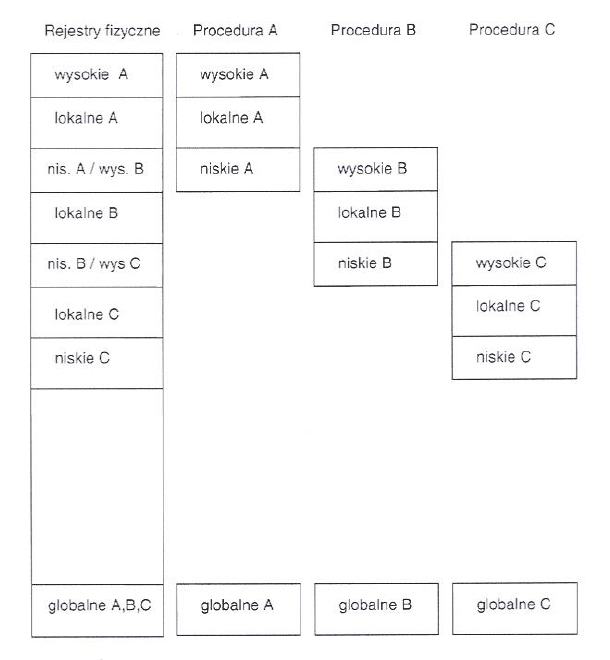
\includegraphics[width=10cm]{RISC_proc1}
%	    \end{center}
%	    \begin{center}
%	    	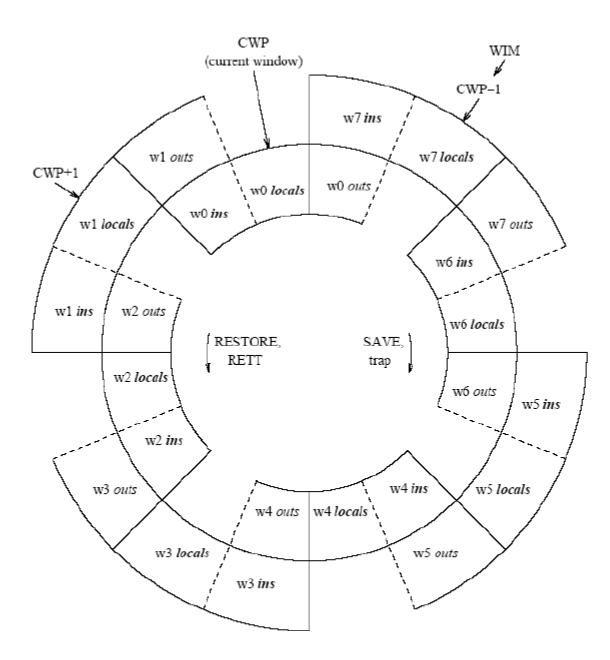
\includegraphics[width=10cm]{RISC_proc2}
%	    \end{center}
	    
	\pagebreak
	\section*{Mechanizmy potokowe}
		\subsection*{Realizacja rozkazów w procesorze niepotokowym}
		Rozkazy wykonywane są liniowo w czasie - jeden po drugim, w takiej kolejności w jakiej przyjdą do procesora.
    	\subsection*{Potokowe wykonanie rozkazówdla prostej organizacji cyklu rozkazowego}
    	Prosty podział procesora na moduły:
    	\begin{itemize}
    		\item S1 - pobranie rozkazu
    		\item S2 - wykonanie rozkazu
    	\end{itemize}
    	Zakładając, że czas pracy obu modułów jest równy, wówczas 3 rozkazy mogą zostać wykonane w 2 okresach.\\
    	1 T - pobranie i wykonanie rozkazu. W momencie gdy pierwszy rozkaz zostanie pobrany, w chwili 0.5 T S1 może pobrać kolejny.
    	\subsection*{Podział cyklu rozkazowego na większą liczbę faz}
    	Na przykładzie cyklu rozkazowego komputera Amdahl 470
    	\begin{enumerate}
    		\item Pobranie rozkazu
    		\item Dekodowanie rozkazu
    		\item Obliczenie adresu efektywnego
    		\item Pobranie argumentów
    		\item Wykonanie operacji
    		\item Zapis wyniku
    	\end{enumerate}
    	Zasada działania jest dokładnie taka sama jak w przypadku podziału na dwie fazy. Załóżmy, że jeden rozkaz wykonuje się w 7iu taktach zegarowych. 1 T = 7 F. Wówczas w momencie gdy rozkaz numer 1 znajduje się w 5tym takcie wykonania rozkaz numer 5 może zostać pobrany.
    	% Table generated by Excel2LaTeX from sheet 'Arkusz1'
    	\begin{table}[htbp]
    		\centering
    		\caption{Zobrazowanie potoku}
    		\begin{tabular}{|r|r|r|r|r|r|r|r|r|}
    			\multicolumn{1}{r}{Rozkazy} & \multicolumn{1}{r}{} & \multicolumn{7}{c}{Fazy zegarowe} \\
    			\multicolumn{1}{r}{} & \multicolumn{1}{r}{} & \multicolumn{1}{c}{1} & \multicolumn{1}{c}{2} & \multicolumn{1}{c}{3} & \multicolumn{1}{c}{4} & \multicolumn{1}{c}{5} & \multicolumn{1}{c}{6} & \multicolumn{1}{c}{7} \bigstrut[b]\\
    			\cline{1-1}\cline{3-9}    \multicolumn{1}{|c|}{S1} &       & r1    & r2    & r3    & r4    & r5    & r6    & r7 \bigstrut\\
    			\cline{1-1}\cline{3-9}    \multicolumn{1}{|c|}{S2} &       &       & r1    & r2    & r3    & r4    & r5    & r6 \bigstrut\\
    			\cline{1-1}\cline{3-9}    \multicolumn{1}{|c|}{S3} &       &       &       & r1    & r2    & r3    & r4    & r5 \bigstrut\\
    			\cline{1-1}\cline{3-9}    \multicolumn{1}{|c|}{S4} &       &       &       &       & r1    & r2    & r3    & r4 \bigstrut\\
    			\cline{1-1}\cline{3-9}    \multicolumn{1}{|c|}{S5} &       &       &       &       &       & r1    & r2    & r3 \bigstrut\\
    			\cline{1-1}\cline{3-9}    \multicolumn{1}{|c|}{S6} &       &       &       &       &       &       & r1    & r2 \bigstrut\\
    			\cline{1-1}\cline{3-9}    \end{tabular}%
    		\label{tab:addlabel}%
    	\end{table}%
    	\subsection*{Analiza czasowa potokowej realizacji ciągu rozkazów}
    	Założenia
    	\begin{itemize}
    		\item \textbf{P} - liczba faz
    		\item \textbf{T} - okres
    		\item $\frac{T}{P}=\tau $ - czas wykonania pojedynczej fazy
    	\end{itemize}
    	$(n-1)\times\tau$ - czas rozpoczęcia wykonywania \emph{n}-tego rozkazu.
    	\subsection*{Czas wykonywania rozkazów}
    	\begin{itemize}
    		\item W procesorze niepotokowym\\
    		$t=n\times T$ - dla \emph{n} rozkazów
    		\item W procesorze potokowym dla idealnego przypadku, gdy $\tau=\frac{T}{P}$\\
    		$t=(n-1)\times\tau=(n-1+P)\times\frac{T}{P}$
    	\end{itemize}
    	\subsection*{Przyspieszenie dla potokowego wykonania rozkazów}
    	Przyspieszenie jest stosunkiem czasu wykonywania rozkazów dla procesora niepotokowego do czasu dla procesora potokowego.\\\\
    	$\lim_{n \to \infty}\frac{n\times T}{(n-1+P)\times\frac{T}{P}}=P$\\\\
    	Maksymalne przyspieszenie (dla modelu idealnego) jest równe ilości faz.
    	\subsection*{Problemy z potokową realizacją rozkazów}
    	Problemem związanym z realizacją potokową jest \textbf{zjawisko hazardu}.
    	\begin{itemize}
    		\item \textbf{Hazard sterowania }– problemy z potokową realizacją skoków i rozgałęzień.
    		\item \textbf{Hazard danych} – zależności między argumentami kolejnych rozkazów
    		\item \textbf{Hazard zasobów} – konflikt w dostępie do rejestrów lub do pamięci
    	\end{itemize}
    	\subsection*{Rozwiązanie problemu hazardu}
    	\begin{itemize}
    		\item Skoki opóźnione
    		\item Przewidywanie rozgałęzień
    	\end{itemize}
    	\subsection*{Skoki opóźnione}
    	\subsubsection*{Założenia}
    	\begin{itemize}
    		\item Rozkaz następny po skoku jest zawsze całkowicie wykonywany
    		\item To znaczy, że efekt skoku jest opóźniony o jeden rozkaz
    	\end{itemize}
    	\subsubsection*{Działanie}
    	Zmienia kod programu w trakcie kompilacji, jeśli widzi taka potrzebę. Sprowadza się to do dwóch możliwości:
    	\begin{itemize}
    		\item Modyfikacji programu - dodanie rozkazu NOP po instrukcji skoku JMP
    		\item Optymalizacji programu - zmiany kolejności wykonywania rozkazów
    	\end{itemize}
    	\subsection*{Przewidywanie rozgałęzień}
    	\begin{enumerate}
    		\item Strategie statyczne
    		\begin{itemize}
    			\item przewidywanie, że rozgałęzienie (skok warunkowy) zawsze nastąpi
    			\item przewidywanie, że rozgałęzienie nigdy nie nastąpi
    			\item podejmowanie decyzji na podstawie kodu rozkazu rozgałęzienia (specjalny bit ustawiany przez kompilator)
    		\end{itemize}
    		\item Inne strategie
    		\begin{itemize}
    			\item przewidywanie, że skok wstecz względem licznika rozkazów zawsze nastąpi
    			\item przewidywanie, że skok do przodu względem licznika rozkazów nigdy nie nastąpi
    		\end{itemize}
    		\item Strategie dynamiczne
    		\begin{itemize}
    			\item Tablica historii rozgałęzień.
    		\end{itemize}
    		\subsubsection*{Tablica historii rozgałęzień}
    		Składa się z:
    		\begin{itemize}
    			\item Bit ważności
    			\item Adres rozkazu rozgałęzienia
    			\item Bity historii
    			\item Adres docelowy rozgałęzienia (opcja)
    		\end{itemize}
    		Operacje wykonywane na tablicy historii rozgałęzień
    		\begin{itemize}
    			\item Sprawdzenie, czy adres rozkazu rozgałęzienia jest w tablicy
    			\begin{itemize}
    				\item \textbf{Nie} – wtedy:
    				\begin{itemize}
    					\item przewidywanie rozgałęzienia jest wykonywane według jednej ze strategii statycznych
    					\item do tablicy jest wpisywany adres rozkazu rozgałęzienia, informacja o wykonaniu/niewykonaniu rozgałęzienia (bit historii) i (opcjonalnie) adres docelowy rozgałęzienia
    				\end{itemize}
    				\item \textbf{Tak} - wtedy:
    				\begin{itemize}
    					\item przewidywanie rozgałęzienia jest wykonywane według bitów historii
    					\item do tablicy jest wpisywana informacja o wykonaniu/niewykonaniu rozgałęzienia (uaktualnienie bitów historii)
    				\end{itemize}
    			\end{itemize}
    			\item 1 bit historii - algorytm przewidywania rozgałęzień dla jednego bitu historii - kolejne wykonanie rozkazu rozgałęzienia będzie przebiegało tak samo jak poprzednie.
    			\item 2 bity historii
    			\begin{itemize}
    				\item algorytm przewidywania rozgałęzień dla dwóch bitów historii bazuje na 2-bitowym automacie skończonym.
    				\item Interpretacja dwóch bitów historii (x y):
    				\begin{itemize}
    					\item y: historia ostatniego wykonania skoku (0 – nie, 1 – tak)
    					\item x: przewidywanie następnego wykonania skoku (0 – nie, 1 – tak)
    					\item Ogólna zasada przewidywania - zmiana strategii następuje dopiero po drugim błędzie przewidywania.
    				\end{itemize}
    			\end{itemize}
    		\end{itemize}
    	\end{enumerate}
   \subsection*{Metody rozwiązywania hazardu danych}
	   \subsubsection*{Co to jest?}
	   Hazard danych - zależności między argumentami kolejnych rozkazów wykonywanych potokowo.
	   \subsubsection*{Metody usuwania hazardu danych}
	   Jest kilka sposobów:
	   \begin{itemize}
	   		\item Sprzętowe wykrywanie zależności i wstrzymanie napełniania potoku
	   		\item Wykrywanie zależności na etapie kompilacji i modyfikacja programu (np. dodanie rozkazu NOP)
	   		\item Wykrywanie zależności na etapie kompilacji, modyfikacja i optymalizacja programu (np. zamiana kolejności wykonywania rozkazów)
	   		\item Wyprzedzające pobieranie argumentów (zastosowanie szyny zwrotnej)
	   \end{itemize}
	   \subsubsection*{Problem}
		Jeśli faza wykonania rozkazu nie będzie mogła być wykonana w jednym takcie (np. dla rozkazów zmiennoprzecinkowych), to zachodzi konieczność wstrzymania napełniania potoku.
	        	
	
    \section*{Architektura superskalarna}
	    \subsection*{Co to jest?}
	    Architektura umożliwiająca wykonanie w jednym takcie większej od 1 liczby instrukcji.
    	\subsection*{Cechy architektury superskalarnej}
        	\begin{itemize}
            \item Możliwość wykonania kilku rozkazów w jednym takcie, co powoduje konieczność:
	            \begin{itemize}
	            	\item Kilku jednostek potokowych
	            	\item Załadowania kilku rozkazów z pamięci operacyjnej w jednym takcie procesora
	            \end{itemize}
	        
            \end{itemize}
		
        \subsection*{Zależności między rozkazami}
        	\begin{itemize}
	            \item \textbf{Prawdziwa zależność danych} - \emph{Read After Write (RAW)}\\
	            Występuje w momencie kiedy jeden rozkaz wymaga argumentu obliczanego przez poprzedni rozkaz. Opóźnienie eliminowane za pomocą "wyprzedzającego pobierania argumentu" - dana nie jest zapisywana do rejestru, tylko pobierana bezpośrednio z 
	            \item \textbf{Zależność wyjściowa} - \emph{Write After Write (WAW)}\\
	            Gdy rozkazy zapisująca dane do tego samego rejestru wykonują się równolegle to drugi z nich musi czekać aż pierwszy się zakończy. Układ sterujący musi kontrolować tego typu zależność.
	            \item \textbf{Antyzależność} - \emph{Write After Read (WAR)}\\
	            W przypadku gdy pierwszy rozkaz czyta wartość rejestru, a drugi zapisuje coś do tego rejestru i oba wykonują się równolegle, to drugi musi czekać aż pierwszy odczyta swoje.
            \end{itemize}
            \subsubsection*{Wnioski}
            \begin{itemize}
            	\item Dopuszczenie do zmiany kolejności rozpoczynania wykonania (wydawania) rozkazów i / lub zmiany kolejności kończenia rozkazów prowadzi do możliwości wystąpienia zależności wyjściowej lub antyzależności.
            	\item Zawartości rejestrów nie odpowiadają wtedy sekwencji wartości, która winna wynikać z realizacji programu
            \end{itemize}
            
		\subsection*{Metody eliminacji zależności}
			\begin{enumerate}
				\item Metoda przemianowania rejestrów
				\begin{itemize}
					\item Stosowana w przypadku zwielokrotnienia zestawu rejestrów.
					\item Rejestry są przypisywane dynamicznie przez procesor do rozkazów.
					\item Gdy wynik rozkazu ma być zapisany do rejestru Rn, procesor angażuje do tego nową kopię tego rejestru.
					\item Gdy kolejny rozkaz odwołuje się do takiego wyniku (jako argumentu źródłowego), rozkaz ten musi przejść przez proces przemianowania.
					\item Przemianowanie rejestrów eliminuje antyzależność i zależność wyjściową.
				\end{itemize}
			\end{enumerate}
			
	\section*{Architektura VLIW}
		\subsection*{Co to jest?}
		VLIW - Very Long Instruction Word.
		\subsection*{Cechy}
		\begin{itemize}
			\item Wspólna pamięć operacyjna
			\item Szeregowanie rozkazów
		\end{itemize}
		\subsection*{Szeregowanie rozkazów przez kompilator}
		\begin{itemize}
			\item Podział rozkazów programu na grupy
			\item Sekwencyjne wykonywanie grup
			\item Możliwość równoległej realizacji rozkazów w ramach grupy
			\item Podział grupy na paczki
			\item Paczka = 3 rozkazy + szablon (3 x 41 + 5 = 128 bitów)
			\item Szablon - informacja o jednostkach funkcjonalnych, do których kierowane mają być rozkazy i ewentualna informacja o granicach grup w ramach paczki
		\end{itemize}
		\subsection*{Redukcja skoków warunkowych - predykacja rozkazów}
		Rozkazy uwarunkowane - uwzględnianie warunku w trakcie realizacji rozkazu.
		\subsection*{Spekulatywne wykonanie rozkazów LOAD}
		\begin{itemize}
			\item Problem: chybione odwołania do PaP (cache) i konieczność czekania na sprowadzenie do PaP linii danych
			\item Rozwiązanie: przesunięcie rozkazów LOAD jak najwyżej, aby zminimalizować czas ewentualnego oczekiwania.
			\item Rozkaz CHECK sprawdza wykonanie LOAD (załadowanie rejestru)
		\end{itemize}
		
	\section*{Wielowątkowość}
		\subsection*{Co to jest?}
		\begin{itemize}
			\item Cecha systemu operacyjnego umożliwiająca wykonywanie kilku wątków w ramach jednego procesu
			\item Cecha procesora oznaczająca możliwość jednoczesnego wykonywanie kilku wątków w ramach jednego procesora (rdzenia)
		\end{itemize}
		\subsection*{Sprzętowa realizacja wielowątkowości}
		Celem współbieżnej realizacji dwóch (lub więcej) wątków w jednym procesorze (rdzeniu) jest minimalizacja strat cykli powstałych w trakcie realizacji pojedynczego wątku w wyniku:
		\begin{itemize}
			\item chybionych odwołań do pamięci podręcznej,
			\item błędów w przewidywaniu rozgałęzień,
			\item zależności między argumentami kolejnych rozkazów
		\end{itemize}
		\subsection*{Wielowątkowość gruboziarnista}
		Coarse-grained multithreading
		\begin{itemize}
			\item Przełączanie wątków następuje przy dłuższym opóźnieniu wątku w potoku (np. chybione odwołanie do pamięci podręcznej (nawet L2))
			\item W niektórych rozwiązaniach rozpoczęcie nowego wątku następuje dopiero po opróżnieniu potoku
			\item Zaletą jest prostota procesu przełączania wątków
			\item Wadą takiego rozwiązania są straty czasu przy krótszych opóźnieniach potoku
		\end{itemize}
		\subsection*{Wielowątkowość drobnoziarnista}
		Fine-grained multithreading
		\begin{itemize}
			\item Przełączanie wątków następuje po każdym rozkazie
			\item Wątek oczekujący (np. na dostęp do pamięci) jest pomijany
			\item Zaletą jest unikanie strat nawet przy krótkich opóźnieniach wątków
			\item Istotnym wymaganiem dla procesora jest szybkie (w każdym takcie) przełączanie wątków
			\item Pewną wadą jest opóźnienie realizacji wątków w pełni gotowych do wykonania
		\end{itemize}
		\subsection*{Warunki sprzętowej realizacji wielowątkowości}
		\begin{itemize}
			\item powielenie zestawów rejestrów uniwersalnych (lub powielenie tabel mapowania rejestrów)
			\item powielenie liczników rozkazów
			\item powielenie układów dostępu do pamięci podręcznej (tabel stron)
			\item powielenie sterowników przerwań
		\end{itemize}
		\subsection*{Wielowątkowość w procesorze dwupotokowym}
		Reguły realizacji i przełączania wątków:
		\begin{enumerate}
			\item Wielowątkowość gruboziarnista
			\begin{itemize}
				\item wątek realizowany w kolejnych taktach do momentu wstrzymania rozkazu
				\item do obu potoków wprowadzane są rozkazy tylko jednego wątku (w jednym takcie!)
			\end{itemize}
			\item Wielowątkowość drobnoziarnista
			\begin{itemize}
				\item w kolejnych taktach realizowane są naprzemiennie rozkazy kolejnych wątków (przełączanie wątków co takt)
				\item do obu potoków wprowadzane są rozkazy tylko jednego wątku (w jednym takcie!)
			\end{itemize}
			\item Wielowątkowość współbieżna (SMT -Simultaneous multithreading)
			\begin{itemize}
				\item wątek realizowany do momentu wstrzymania rozkazu
				\item do obu potoków w jednym takcie mogą być wprowadzane rozkazy różnych wątków
			\end{itemize}
		\end{enumerate}
		\subsection*{Mankamenty współbieżnej wielowątkowości}
		\begin{itemize}
			\item Rywalizacja wątków w dostępie do pamięci podręcznej - mniejsza wielkość PaP przypadająca na wątek
			\item Większe zużycie energii (w porównaniu z procesorami dwurdzeniowymi)
			\item Możliwość monitorowanie wykonania jednego wątku przez inny wątek (złośliwy), poprzez wpływ na współdzielone dane pamięci podręcznej - kradzież kluczy kryptograficznych
		\end{itemize}
	
	\section*{Klasyfikacja komputerów równoległych}
		\subsection*{Formy równoległości w architekturze komputerów}
			\subsubsection*{Równoległość na poziomie rozkazów}
			Wykonywanie w danej chwili wielu rozkazów w jednym procesorze.
			\begin{itemize}
				\item Mechanizmy potokowe - w procesorach CISC i RISC
				\item Architektura superskalarna i VLIW
			\end{itemize}
			\subsubsection*{Równoległość na poziomie procesorów}
			Wykonywanie w danej chwili wielu rozkazów w wielu procesorach.
			\begin{itemize}
				\item Komputery wektorowe
				\item Komputery macierzowe
				\item Systemy wieloprocesorowe
				\item Klastry (systemy wielokomputerowe)
			\end{itemize}
		\subsection*{Rodzaje równoległości w aplikacjach}
			\subsubsection*{Równoległość poziomu danych}
			DLP - Data Level Parallelism.\\
			Pojawia się kiedy istnieje wiele danych, które mogą być przetwarzane w tym samym czasie.
			\subsubsection*{Rówoległość poziomu zadań}
			TLP - Task Level Parallelism.\\
			Pojawia się kiedy są tworzone zadania, które mogą być wykonywane niezależnie i w większości równolegle.
		
		\subsection*{Drogi wykorzystania równoległości aplikacji w architekturze komputerów}
			\begin{itemize}
				\item \textbf{Równoległość poziomu rozkazów} (ILP - InstructionLevel Parallelism) - odnosi się do przetwarzania potokowego i superskalarnego, w których w pewnym (niewielkim) stopniu wykorzystuje się równoległość danych.
				\item \textbf{Architektury wektorowe i procesory graficzne} - wykorzystują równoległość danych poprzez równoległe wykonanie pojedynczego rozkazu na zestawie danych.
				\item \textbf{Równoległość poziomu wątków} (TLP - ThreadLevel Parallelism) - odnosi się do wykorzystania równoległości danych albo równoległości zadań w ściśle połączonych systemach (ze wspólną pamięcią), które dopuszczają interakcje między wątkami.
				\item \textbf{Równoległość poziomu zleceń} (RLP - RequestLevel Parallelism) - odnosi się do równoległości zadań określonych przez programistę lub system operacyjny. Ta forma równoległości jest wykorzystywana w systemach luźno połączonych (z pamięcią rozproszoną) i klastrach.
			\end{itemize}
			
		\subsection*{Klasyfikacja Flynna}
		M. Flynn, 1966
		\subsubsection*{Kryterium klasyfikacji}
		Liczba strumieni rozkazów i liczba strumieni danych w systemie komputerowym
		\begin{itemize}
			\item SISD: Single Instruction, Single Data Stream
			\item SIMD: Single Instruction, Multiple Data Stream
			\item MISD: Multiple Instruction, Single Data Stream
			\item MIMD: Multiple Instruction, Multiple Data Stream
		\end{itemize}
		\subsubsection*{Klasyfikacja opisowa}
		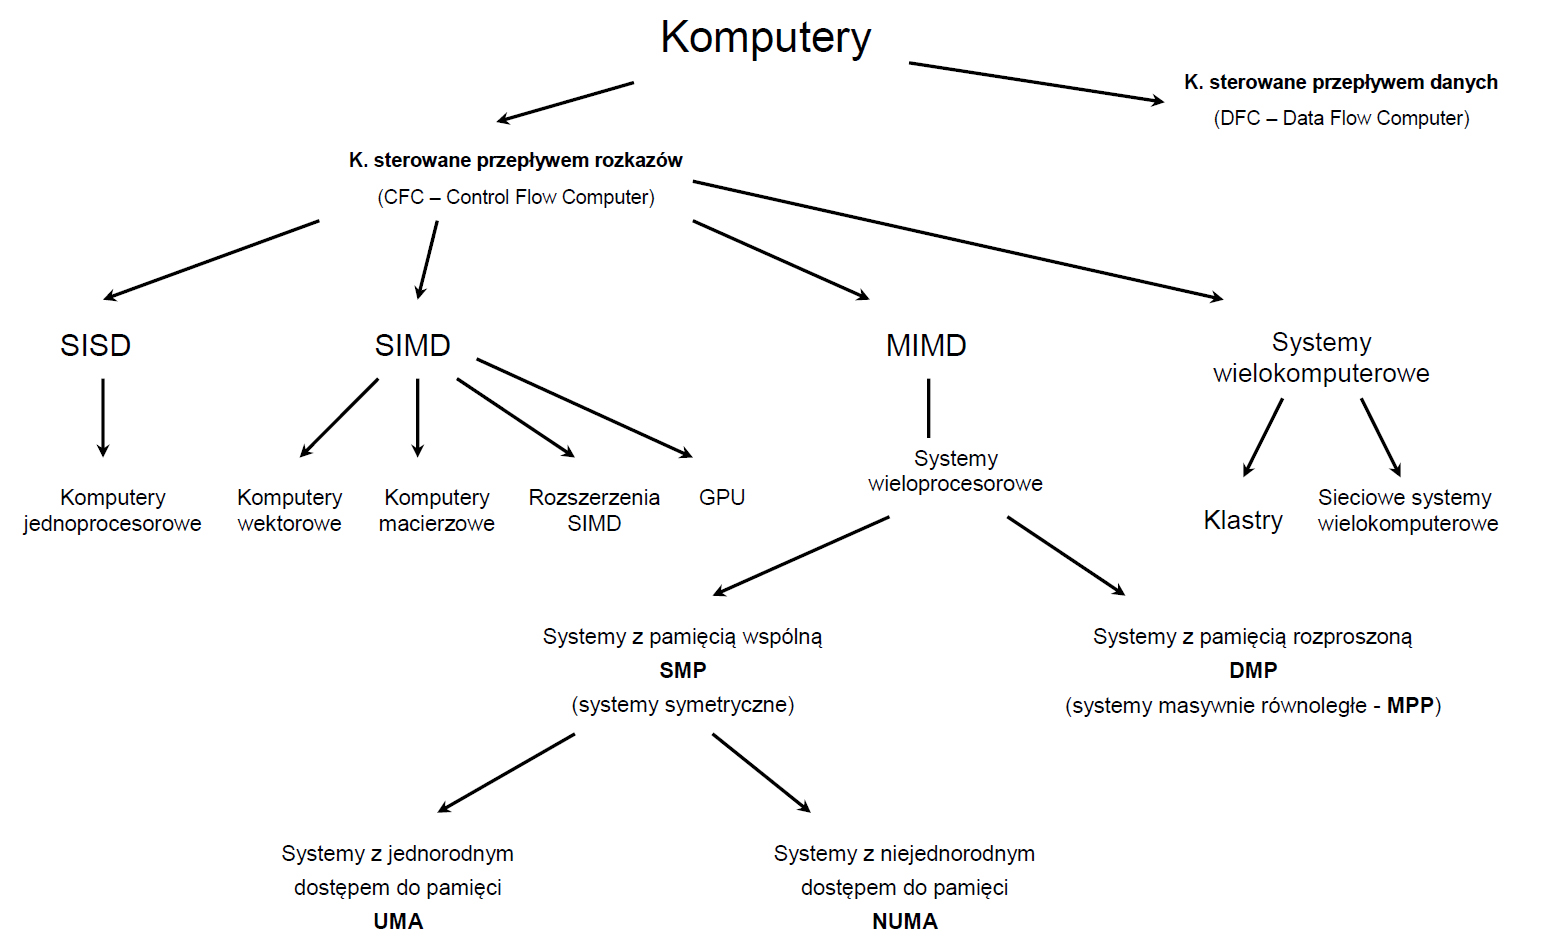
\includegraphics[width=16cm]{klasyfikacja}
		\pagebreak
		
	\section*{Architektura SIMD}
		\subsection*{Co to jest?}
		Cecha wyróżniająca dla programisty - rozkazy wektorowe (rozkazy z argumentami wektorowymi).\\
		Dwa różne podejścia do sprzętowej realizacji rozkazów wektorowych:
		\begin{itemize}
			\item Komputery (procesory) macierzowe
			\item Komputery wektorowe
		\end{itemize}
		Idee realizacji obu (macierzowy i wektorowy):\\
		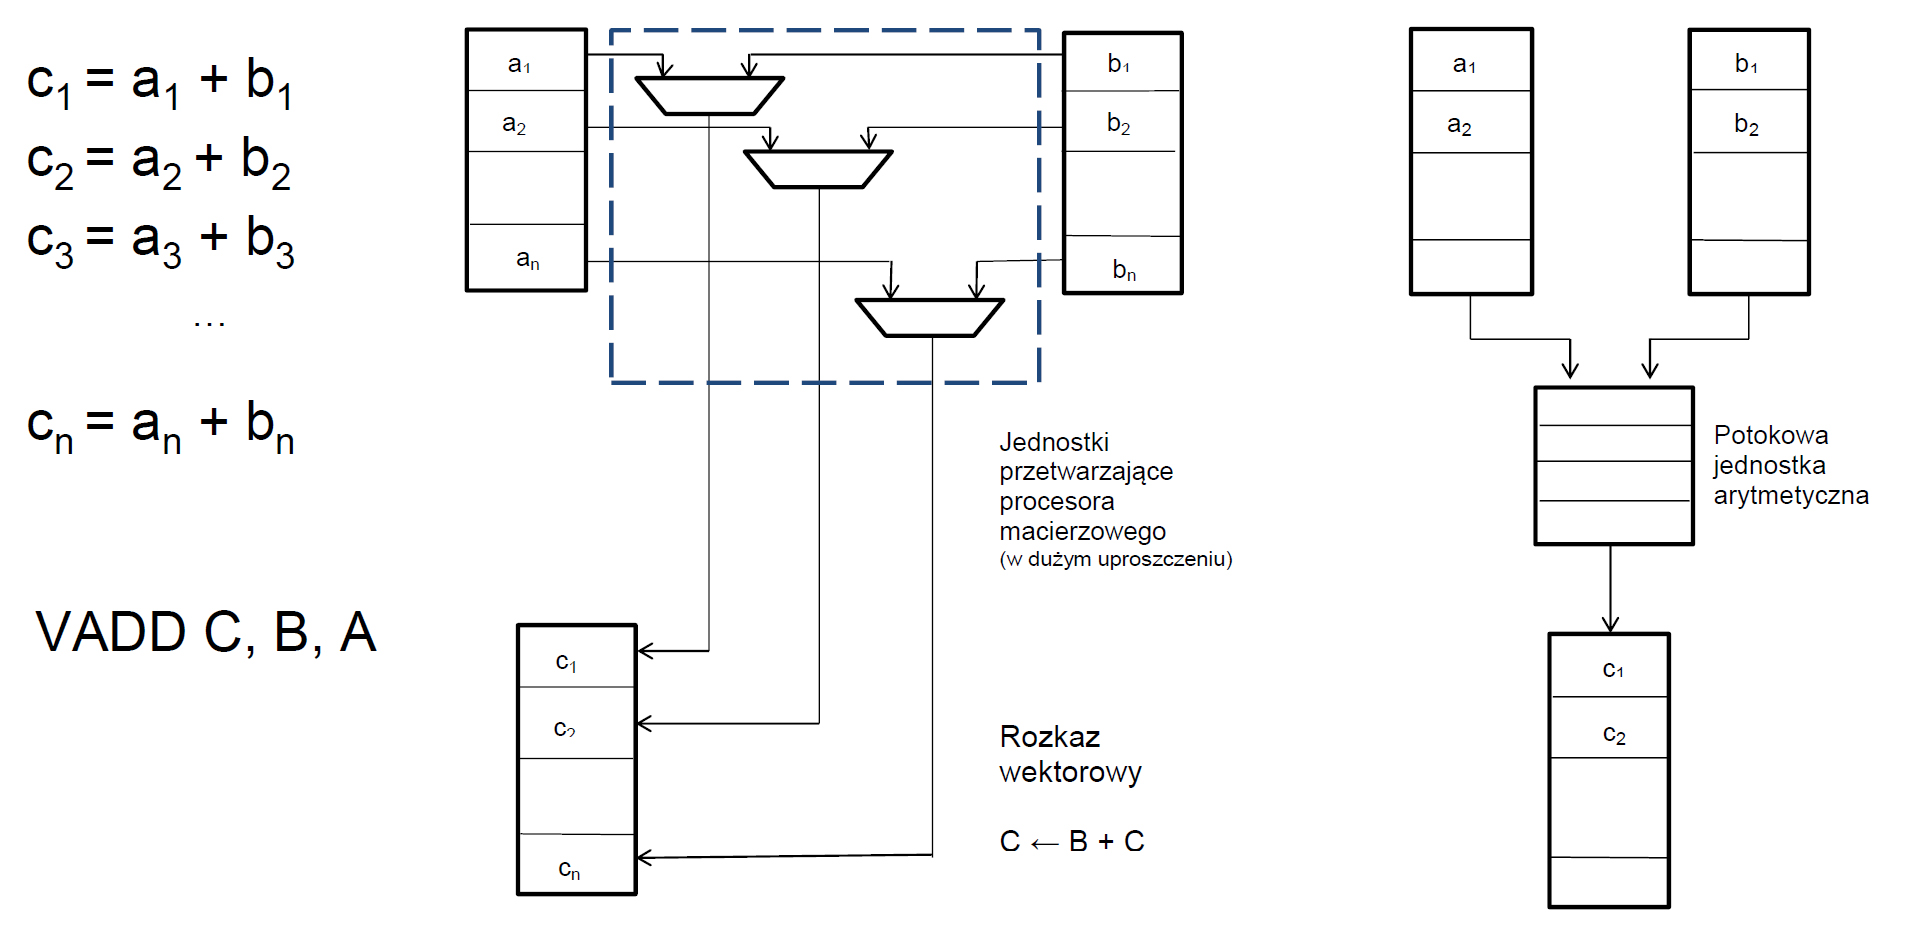
\includegraphics[width=16cm]{wektor_macierz}\\
		\subsection*{Komputery wektorowe}
			\subsubsection*{Lokalizacja wektorów danych}
			\begin{itemize}
				\item Pamięć operacyjna
				\item Rejestry wektorowe
			\end{itemize}
			\subsubsection*{Przykład rozkazu}
			Rozkaz dodawania wektorów: VADDF A,B,C,n\\
			Czas wykonania: $t_{w}=t_{start}+(n-1)\times\tau$\\
			W komputerze macierzowym czas wykonywania tego rozkazu jest równy \emph{const}.
			
			\subsubsection*{Przyspieszenie}
			Przyspieszenie jest stosunkiem czasu wykonywania w komputerze klasycznym (szeregowo) do czasu wykonywania w komputerze wektorowym.\\\\
			$a=lim_{n \to \infty}\frac{15\times\tau\times n}{t_{start}+(n-1)\times\tau}=15$
			
			\subsubsection*{Przepustowość}
			Przepustowość (moc obliczeniowa) jest stosunkiem ilości operacji zmiennoprzecinkowych do czasu ich wykonania.\\\\
			$Przep=lim_{n \to \infty}\frac{n}{t_{start}+(n-1)\times\tau}=\frac{1}{\tau}$
		
			\subsubsection*{Podsumowanie}
				\begin{enumerate}
					\item Hardware
					\begin{itemize}
						\item rozkazy wektorowe
						\item duża liczba potokowych jednostek arytmetycznych
						\item duża liczba rejestrów
					\end{itemize}
					\item Software
					\begin{itemize}
						\item klasyczne języki: Fortran, C
						\item klasyczne algorytmy
						\item kompilatory wektoryzujące
					\end{itemize}
				\end{enumerate}
	
			\subsubsection*{Zastosowanie}
			\begin{itemize}
				\item Numeryczna symulacja ośrodków ciągłych
				\item Równania różniczkowe, równania różnicowe, układy równań algebraicznych (rachunek macierzowy)
				\item Dziedziny zastosowań:
				\begin{itemize}
					\item prognozowanie pogody
					\item symulacja aerodynamiczna
					\item sejsmiczne poszukiwania ropy naftowej i innych surowców
					\item symulacja reakcji jądrowych
					\item medycyna i farmacja
					\item obliczenia inżynierskie dużej skali
				\end{itemize}
			\end{itemize}
			
		\subsection*{Komputery macierzowe}
			\subsubsection*{Co to jest?}
			Architektura komputerów macierzowych - model SIMD w dwóch wariantach:
			\begin{itemize}
				\item SIMD - DM (z pamięcią rozproszoną)
				\item SIMD - SM (z pamięcią wspólną)
			\end{itemize}
			
			\subsubsection*{Elementy komputera macierzowego}
			\begin{enumerate}
				\item \textbf{Jednostka sterująca} - procesor wykonujący rozkazy sterujące i skalarne oraz inicjujący wykonanie rozkazów wektorowych w sieci elementów przetwarzających.
				\item \textbf{Elementy przetwarzające} (procesorowe) - jednostki arytmetyczno-logiczne wykonujące operacje elementarne rozkazów wektorowych.
				\item \textbf{Sieć łącząca} - łączy elementy przetwarzające między sobą lub z modułami pamięci operacyjnej; warianty:
				\begin{itemize}
					\item sieć statyczna: pierścień, gwiazda, krata, drzewo, hipersześcian
					\item sieć dynamiczna: jednostopniowa, wielostopniowa
				\end{itemize}
			\end{enumerate}
			
			\subsubsection*{Podsumowanie}
			\begin{itemize}
				\item Architektura SIMD
				\item Jednostka sterująca + jednostka macierzowa
				\item Rozkazy wektorowe - wykonywane synchronicznie w sieci (macierzy) EP
				\item Skomplikowana wymiana danych między EP
				\item Trudne programowanie - konieczność tworzenia nowych wersji algorytmów
			\end{itemize}
			
		\subsection*{Model SIMD w procesorach superskalarnych}
			\subsubsection*{Technologia MMX}
			\begin{itemize}
				\item 8 rejestrów 64-bitowych MMX
				\item Nowe typy danych
				\item Rozszerzony zestaw instrukcji (57 instrukcji)
				\item Realizacja operacji na krótkich wektorach wg modelu SIMD
			\end{itemize}
			\subsection*{Technologia SSE}
			\begin{itemize}
				\item 8 rejestrów 128-bitowych
				\item Osiem 16-bitowych argumentów (elementów wektora) typu integer
				\item Cztery 32-bitowe argumenty integer/fplub dwa 64-bitowe
				\item Operacje zmp na 4-elementowych wektorach liczb 32-bit (pojed. prec.)
			\end{itemize}
			
	\section*{Karty graficzne i architektura CUDA}
		\subsection*{Charakterystyka}
		\begin{itemize}
			\item GPU - Graphics Processing Unit
			\item Wcześniejsze GPU - specjalizowane języki (HLSL, GLSL czy NVIDIA Cg), tylko rendering
			\item CUDA (Compute Unified Device Architecture) -architektura wielordzeniowych procesorów graficznych (GPU)
			\item Uniwersalna architektura obliczeniowa połączona z równoległym modelem programistycznym
			\item wsparcie dla języków C/C++
			\item GPGPU = GPU + CUDA
			\item CUDA - obsługiwana przez karty graficzne GeForce i GeForce Mobile od serii 8 (GeForce 8800), nowsze układy z rodzin Tesla i Quadro, Fermi, obecnie Kepler
		\end{itemize}
		\subsection*{Architektura CUDA}
		\begin{itemize}
			\item W miejsce oddzielnych potoków przetwarzających wierzchołki i piksele wprowadzenie uniwersalnego procesora przetwarzającego wierzchołki, piksele i ogólnie geometrię, a także uniwersalne programy obliczeniowe
			\item Wprowadzenie procesora wątków eliminującego „ręczne” zarządzanie rejestrami wektorowymi
			\item Wprowadzenie modelu SIMT (single-instruction multiple-thread), w którym wiele niezależnych wątków wykonuje równocześnie tę samą instrukcję
			\item Wprowadzenie współdzielonej pamięci oraz mechanizmów synchronizacji wątków (barrier synchronization) dla komunikacji między wątkami
		\end{itemize}
		\subsection*{Multiprocesor strumieniowy}
		\begin{itemize}
			\item 8 rdzeni C1 -C8 (SP)
			\item podręczna pamięć instrukcji (ang. instruction cache),
			\item podręczna pamięć danych (ang. constant cache) -pamięć tylko do odczytu,
			\item pamięć współdzielona (ang. shared memory)
			\item 16 384 rejestry,
			\item jednostka arytmetyczna wykonująca obliczenia zmiennoprzecinkowe podwójnej precyzji (fp64),
			\item dwie jednostki arytmetyczne przeznaczone do obliczania funkcji specjalnych (ang. special function unit),
			\item pamięć globalna
		\end{itemize}
		\subsection*{Model programistyczny CUDA}
		\begin{itemize}
			\item Specjalny kompilator NVCC
			\item Podział programu na kod wykonywany przez procesor (ang. Host code) i przez urządzenie (kartę graficzną) (ang. Device code) - kernel
			\item Realizacja operacji równoległych według modelu SIMT (Single Instruction Multiple Threading)
		\end{itemize}
		\subsection*{Wykonanie obliczeń z użyciem architektury CUDA (5 faz)}
		\begin{enumerate}
			\item Przydzielenie w pamięci globalnej obszaru pamięci dla danych, na których będą wykonywane obliczenia przez kernel.
			\item Przekopiowanie danych do przydzielonego obszaru pamięci.
			\item Zainicjowanie przez CPU obliczeń wykonywanych przez GPU, tj. wywołanie kernela.
			\item Wykonanie przez wątki (z użyciem GPU) obliczeń zdefiniowanych w kernelu.
			\item Przekopiowanie danych z pamięci globalnej do pamięci operacyjnej.
		\end{enumerate}
		\subsection*{CUDA procesor (rdzeń)}
		\begin{itemize}
			\item Potokowa jednostka arytmetyczna zmp
			\item Potokowa jednostka arytmetyczna stp
			\item Ulepszona realizacja operacji zmp FMA (fused multiply-add) dla pojedynczej i podwójnej precyzji
		\end{itemize}
		\pagebreak
		\section*{Wątki}
			\begin{itemize}
				\item Wątek reprezentuje pojedynczą operację (a single work unit or operation)
				\item Wątki są automatycznie grupowane w bloki, maksymalny rozmiar bloku = 512 wątków (w architekturze Fermi i wyższych –1024 wątki).
				\item Bloki grupowane są w siatkę (grid -kratę)
				\item Grupowanie wątków –bloki o geometrii 1, 2 lub 3-wymiarowej
				\item Grupowanie bloków –siatka (grid) o geometrii 1, 2-wymiarowej
				\item Wymaga się, aby bloki wątków tworzących siatkę mogły się wykonywać niezależnie: musi być możliwe ich wykonanie w dowolnym porządku, równolegle lub szeregowo.
			\end{itemize}
			\subsection*{Grupowanie wątków w bloki i siatkę}
			\begin{itemize}
				\item Siatka o geometrii jednowymiarowej (trzy bloki wątków)
				\item Każdy blok -geometria dwuwymiarowa (wymiary 2 x 3)
			\end{itemize}
			\subsection*{Sprzętowa organizacja wykonywania wątków}
				\begin{itemize}
					\item Przy uruchomieniu kernel’awszystkie bloki tworzące jego siatkę obliczeń są rozdzielane pomiędzy multiprocesory danego GPU
					\item Wszystkie wątki danego bloku są przetwarzane w tym samym multiprocesorze
					\item W danej chwili (cyklu) pojedynczy rdzeń multiprocesora wykonuje jeden wątek programu
					\item Multiprocesor tworzy, zarządza, szereguje i wykonuje wątki w grupach po 32, nazywanych wiązkami (warp).
					\item Wiązki są szeregowane do wykonania przez warp scheduler. Wiązka wątków jest wykonywana jako jeden wspólny rozkaz (analogia do rozkazu SIMD, tzn. rozkazu wektorowego)
					\item Sposób wykonania wiązki wątków (rozkazu SIMD) zależy od budowy multiprocesora:
					\begin{itemize}
						\item Dla architektury Fermi (32 procesory w jednym multiprocesorze / 2 warp-scheduler’y= 16 procesorów na 1 wiązkę) wiązka jest wykonywana jako 2 rozkazy -wiązka jest dzielona na dwie połówki (half –warp) wykonywane jako 2 rozkazy (te same, ale na dwóch zestawach danych).
						\item Dla architektury Tesla (8 procesorów w jednym multiprocesorze, 1 warp-scheduler) wiązka jest dzielona na cztery ćwiartki (quarter-warp) wykonywane jako 4 kolejne rozkazy (te same, ale na czterech zestawach danych).
					\end{itemize}
					\item Konstrukcja warp scheduler’a umożliwia uruchomienie wielu wiązek wątków współbieżnie - warp scheduler pamięta wtedy adresy wiązek, przypisane im rozkazy SIMD oraz ich stan (gotowość do wykonania lub stan oczekiwania na pobranie danych z pamięci).
					\item Współbieżne uruchomienie wielu wiązek pozwala zmniejszyć straty związane z oczekiwaniem na dane (zwykle długi czas dostępu do pamięci).
				\end{itemize}
				
		\section*{Rodzaje pamięci multiprocesora}
		\begin{itemize}
			\item \textbf{pamięć globalna} – duża pamięć, o czasie życia aplikacji (dane umieszczone w tej pamięci są usuwane po zakończeniu aplikacji), dostępna dla każdego wątku w dowolnym bloku, ale o dość długim czasie dostępu wynoszącym ok. 400-600 taktów zegara,
			\item \textbf{pamięć współdzielona} – niewielka pamięć o czasie życia bloku (zakończenie działania bloku powoduje usunięcie danych w niej przechowywanych), dostępna dla każdego wątku w bloku dla którego jest dedykowana, o bardzo krótkim czasie dostępu,
			\item \textbf{pamięć stałych} – niewielki fragment pamięci globalnej, który jest cache-owany, przez co dostęp do niego jest bardzo szybki. Jest ona tylko do odczytu. Czas życia pamięci stałych oraz jej dostępność jest taka sama jak pamięci globalnej,
			\item \textbf{rejestry} – niewielka, bardzo szybka pamięć o czasie życia wątku (po zakończeniu wątku dane z rejestrów są usuwane). Tylko jeden wątek może w danym momencie korzystać z danego rejestru,
			\item \textbf{pamięć lokalna i pamięć tekstur} – podobnie jak w przypadku pamięci stałych, są to dedykowane fragmenty pamięci globalnej. Pamięć lokalna jest wykorzystywana do przechowywania danych lokalnych wątku, które nie mieszczą się w rejestrach, a pamięć tekstur posiada specyficzne metody adresowania i cache-owanie specyficzne dla zastosowań graficznych.
		\end{itemize}
	
%===============================================================================	
%*******************************************************************************
%===============================================================================
\end{document}